% The next command tells RStudio to do "Compile PDF" on HSB.Rnw,
% instead of this file, thereby eliminating the need to switch back to HSB.Rnw 
% before building the paper.
%!TEX root = ../HSB.Rnw

\begin{landscape}
\begin{table}
\begin{center}
\caption{Comparison among relevant partial equilibrium rebound analysis frameworks.}
\begin{tabular}{r c c c c c c}
  \toprule
                                             & \rot{\citet{Nassen:2009aa}}
                                             & \rot{\citet{Thomas:2013aa,Thomas:2013ab}}
                                             & \rot{\citet{Borenstein:2015aa}}
                                             & \rot{\citet{Chan2015}}
                                             & \rot{\citet{Wang2021}}
                                             & \rot{This paper} \\
  \midrule
  \multicolumn{1}{l}{\emph{Effects, 
                           locations, and scales}}                &                &                &                &                  &               &                \\
  Direct emplacement effect                                       & \rating{100}   & \rating{50}    & \rating{50}    & \rating{50}      & \rating{50}   & \rating{100}   \\
  Capital cost and embodied energy effect                         & \rating{50}    & \rating{50}    & \rating{50}    & \rating{25}      & \rating{0}    & \rating{100}   \\
  Maintenance and disposal effect                                 & \rating{0}     & \rating{0}     & \rating{50}    & \rating{0}       & \rating{0}    & \rating{100}   \\
  Direct and indirect substitution effects                        & \rating{50}    & \rating{50}    & \rating{100}   & \rating{100}     & \rating{100}  & \rating{100}   \\
  Direct and indirect income effects                              & \rating{50}    & \rating{50}    & \rating{100}   & \rating{100}     & \rating{100}  & \rating{100}   \\
  Macro effect                                                    & \rating{0}     & \rating{0}     & \rating{25}    & \rating{0}       & \rating{0}    & \rating{100}   \\
  \midrule
  \multicolumn{1}{l}{\emph{Other characteristics}}                &                &                &                &                  &               &                \\
  Presentation of energy, expenditure, and consumption spaces     & \rating{75}    & \rating{75}    & \rating{50}    & \rating{75}      & \rating{50}   & \rating{100}   \\
  Detailed model of consumer preferences                          & \rating{25}    & \rating{50}    & \rating{50}    & \rating{100}     & \rating{100}  & \rating{100}   \\
  Non-marginal energy service price changes                       & \rating{0}     & \rating{0}     & \rating{0}     & \rating{0}       & \rating{0}    & \rating{100}   \\
  Operationality                                                  & \rating{100}   & \rating{100}   & \rating{50}    & \rating{0}       & \rating{0}    & \rating{100}   \\
\bottomrule
\end{tabular}
\label{tab:previous_frameworks}
\end{center}
\end{table}
\end{landscape}



% \renewcommand{\arraystretch}{1}

% \begin{table} 
%   \caption{Previous rebound analysis frameworks. **** This table is not correct. We need to decide which 
%            frameworks to include and their characteristics. ---MKH ****}
%   \centering
%   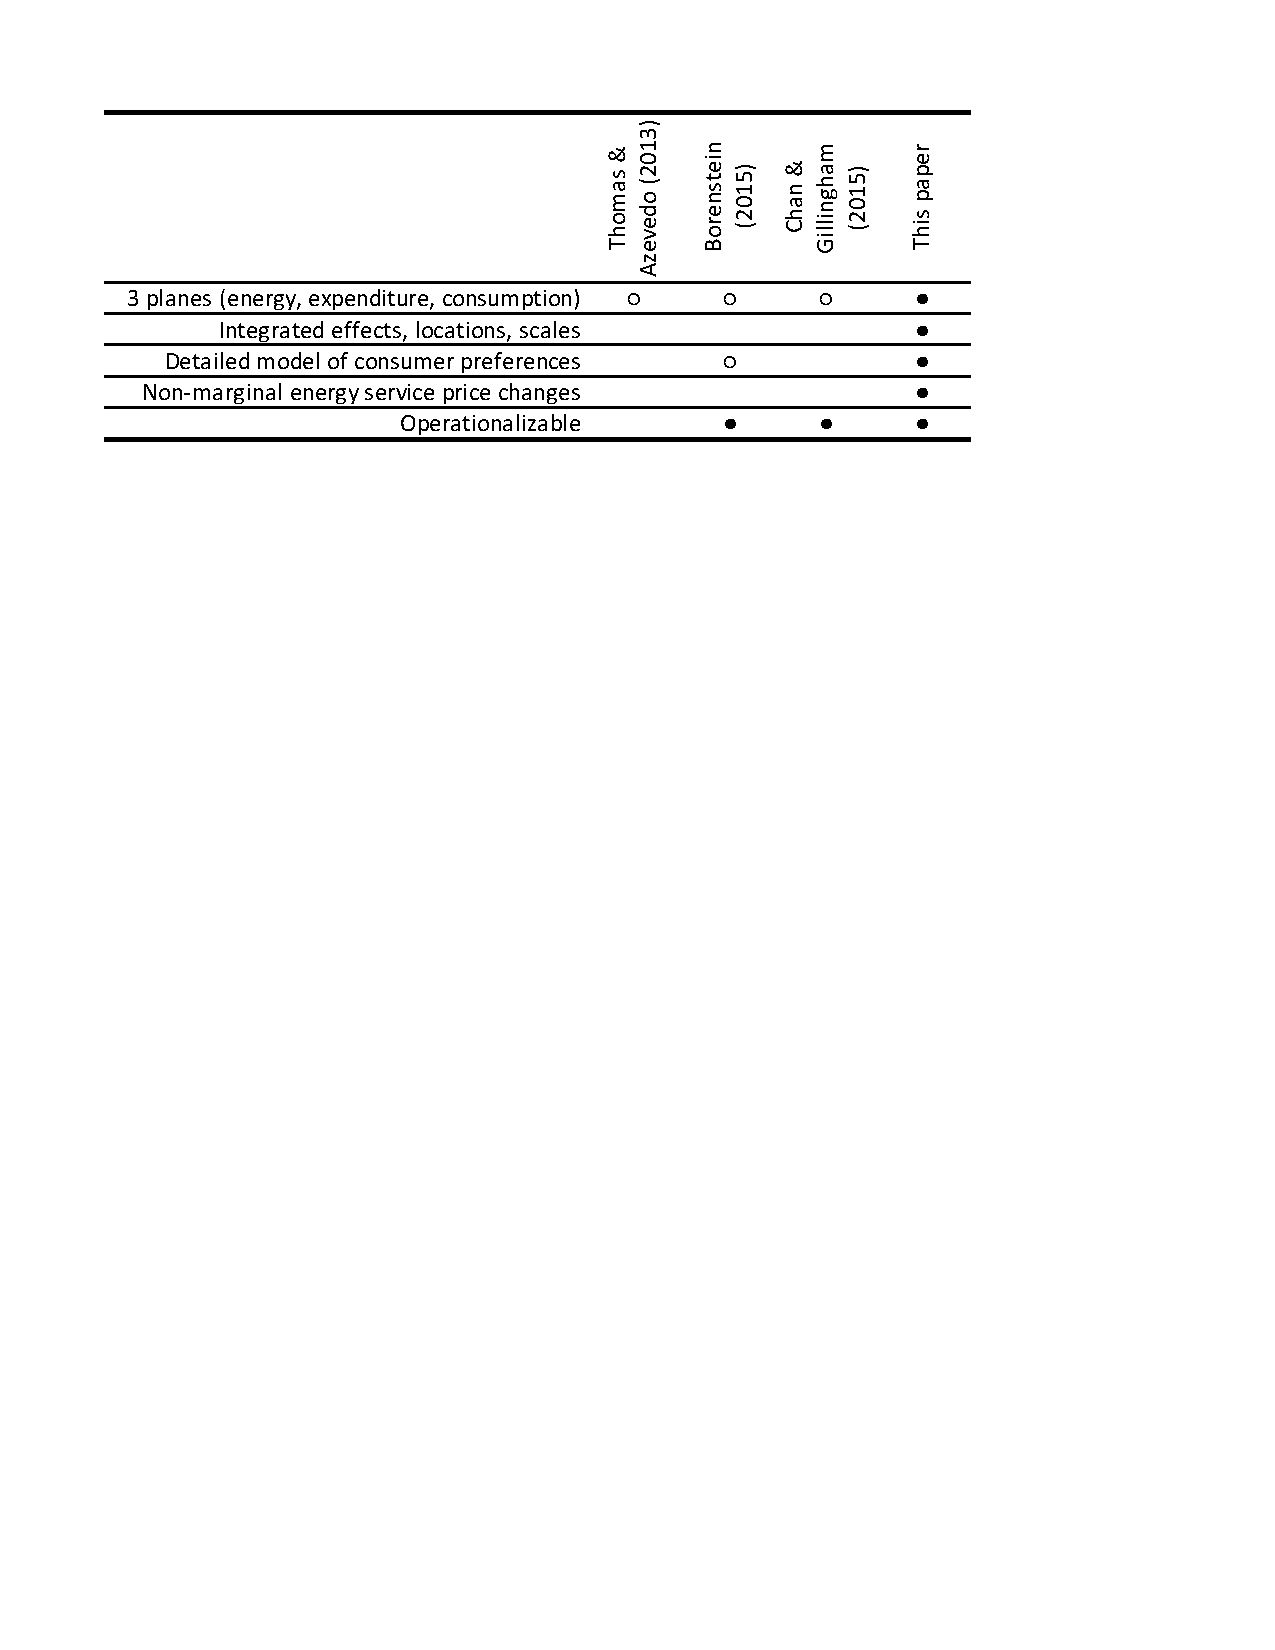
\includegraphics[width=1\linewidth]{figure_other/PreviousFrameworksTable.pdf}
%   \label{tab:previous_frameworks}
% \end{table}

